% !Mode:: "TeX:UTF-8"

\chapter{两轮平衡车性能测试实验研究}

为验证前文所提出两轮平衡车总体方案及关键技术的有效性，本章从整车运动性能、双目视觉环境感知能力以及自主行驶能力三个方面开展实验研究。首先，通过基本行驶性能测试分析车辆在启动、加减速、转向及越障等典型工况下的姿态稳定性与操控性能；其次，结合嵌入式平台部署与外场测距实验，对双目视觉感知算法的实时性与测距精度进行评估；最后，通过定位效果与动态避障实验，对系统各模块的协同工作效果与整车运行稳定性进行验证，从而为所构建系统的工程可行性与应用可靠性提供实验依据。

\section{两轮平衡车基本行驶性能的测试实验}

为验证两轮平衡车底盘结构设计与平衡控制系统的可靠性，本节从定量指标测试和典型工况观察两个方面开展基本行驶性能测试。

在额定载荷工况下，首先进行最高速度、最大加速度和最大爬坡角测试。最高速度测试在平直水泥路面上进行，测试过程中采集轮毂电机驱动器反馈的转速数据，并结合车轮半径换算得到车辆纵向速度，取速度序列最大值作为最高速度。最大加速度测试采用零初速度起步方式，根据连续采样的速度--时间数据计算相邻采样时刻的速度变化率，并取起步加速阶段的峰值作为最大加速度。最大爬坡角测试采用倾角为$15^\circ$、斜面长度约$1.55\,\mathrm{m}$的斜坡垫进行，车辆从距斜坡垫底端$0.5\,\mathrm{m}$处由静止状态起步，观察其是否能够稳定通过斜坡。

\begin{table}[htbp]
  \centering
  \caption[基本行驶性能定量测试结果]{基本行驶性能定量测试结果}
  \label{基本行驶性能测试结果}
  \vspace{0.5em}\wuhao
  \begin{thesistabular}{cc}
    \toprule
    测试项目 & 实验结果 \\
    \midrule
    最高速度 & $16.47\,\mathrm{km/h}$ \\
    最大加速度 & $3.71\,\mathrm{m/s^2}$ \\
    最大爬坡角 & 可稳定通过$15^\circ$斜坡 \\
    \bottomrule
  \end{thesistabular}
\end{table}

定量测试结果如表\ref{基本行驶性能测试结果}所示。车辆在平直水泥路面上的最高速度达到$16.47\,\mathrm{km/h}$，从静止起步后测得的最大加速度为$3.71\,\mathrm{m/s^2}$，且能够稳定通过$15^\circ$斜坡，达到表\ref{tab:总体设计主要技术指标}中最高速度、最大加速度和最大爬坡角的设计指标。

在定性测试中，车辆在砂石路面上连续进行减速带越障、砖块越障以及绕桩行驶实验，用于观察车辆在典型起伏路面和复杂路径条件下的姿态稳定性与操控连续性。图\ref{行驶能力测试}展示了减速带越障、砖块越障以及绕桩实验的实际测试情况。

\begin{figure}[htbp]
  \centering
  \begin{minipage}[t]{0.32\textwidth}
    \centering
    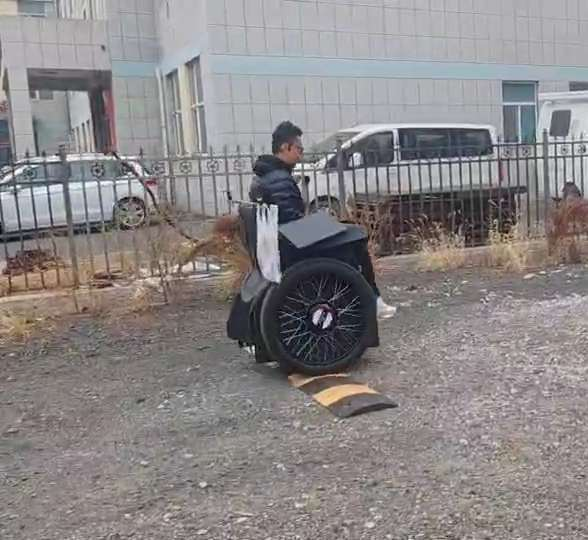
\includegraphics[width=\textwidth]{figures/chapter05/行驶能力测试_1.jpg}
  \end{minipage}
  \hfill
  \begin{minipage}[t]{0.32\textwidth}
    \centering
    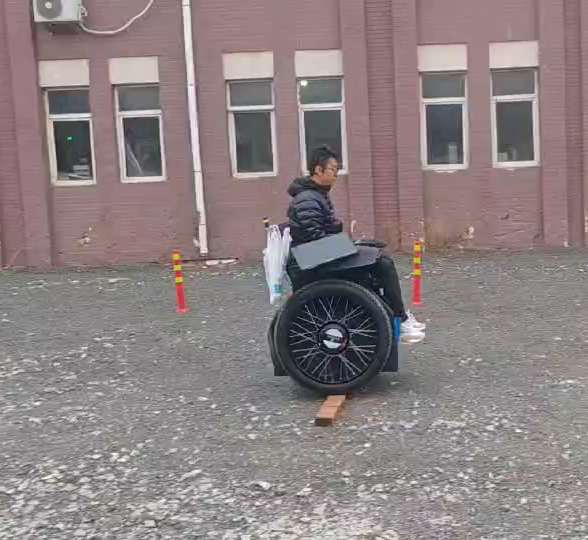
\includegraphics[width=\textwidth]{figures/chapter05/行驶能力测试_2.jpg}
  \end{minipage}
  \hfill
  \begin{minipage}[t]{0.32\textwidth}
    \centering
    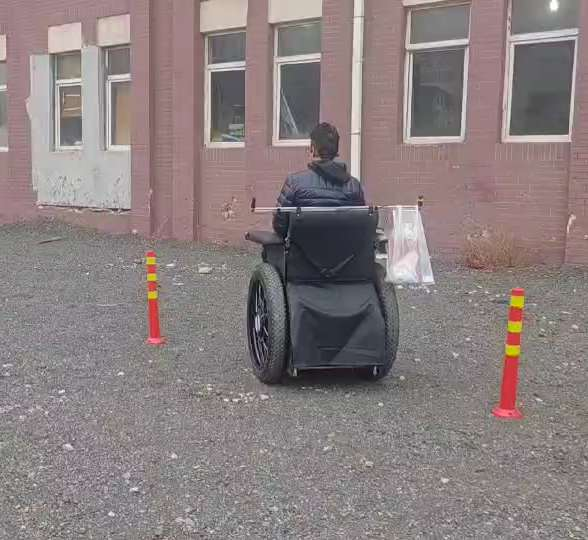
\includegraphics[width=\textwidth]{figures/chapter05/行驶能力测试_3.jpg}
  \end{minipage}
  \caption{行驶能力测试}
  \label{行驶能力测试}
\end{figure}

定性测试结果表明，车辆通过减速带、砖块和绕桩路径时未出现明显失衡、侧倾或姿态超调现象，运行过程整体平稳。上述结果说明车辆具备较好的基本运动能力和地面适应能力，验证了底盘结构与平衡控制系统的可靠性。

\section{双目视觉环境感知算法的测试实验}

\subsection{嵌入式平台部署与加速效果测试}

本节主要验证双目立体匹配与目标检测融合算法在嵌入式平台上的实时性与测距精度，并分析模型部署优化带来的性能提升。

嵌入式部署测试的软硬件环境如表\ref{嵌入式部署实验软硬件环境}所示。测试平台采用前文所述NVIDIA Jetson Orin Nano Super，软件环境基于JetPack 6.3构建，其中深度学习推理加速库采用TensorRT 10.3，模型均在同一平台与相同输入分辨率条件下进行测试，以保证不同部署方式之间具有可比性。

\begin{table}[htbp]
  \centering
  \caption[嵌入式部署实验软硬件环境]{嵌入式部署实验软硬件环境}
  \label{嵌入式部署实验软硬件环境}
  \vspace{0.5em}\wuhao
  \begin{thesistabular}{cc}
    \toprule
    项目 & 配置 \\
    \midrule
    硬件平台 & NVIDIA Jetson Orin Nano Super（8GB） \\
    操作系统与开发套件 & Ubuntu 22.04，JetPack 6.3（L4T 36.4） \\
    GPU计算库 & CUDA 12.6，cuDNN 9.3 \\
    推理加速库 & TensorRT 10.3（FP16） \\
    输入分辨率 & 640$\times$480 \\
    \bottomrule
  \end{thesistabular}
\end{table}

为评估模型在嵌入式平台上的推理性能，分别对YOLO11n目标检测网络与立体匹配网络（HAGVNet）进行了部署测试，对比了PyTorch原生推理与TensorRT加速推理两种方式的性能表现。其中，PyTorch推理作为功能验证与性能基线；TensorRT在模型导出与转换基础上，采用FP16精度模式，并结合算子融合与图优化策略进行端到端加速，从而提升嵌入式设备上的运行效率。

实验结果如表\ref{不同部署方式下的模型推理性能对比}所示，相比PyTorch推理，TensorRT（FP16）显著降低了模型延迟：（1）HAGVNet单帧推理时间由194.3ms降至21.6ms，对应帧率提升至46.3FPS；（2）YOLO11n单帧推理时间由62.3ms降至6.9ms，对应帧率提升至144.9FPS。可以看出，在嵌入式平台上，TensorRT加速对两类模型均带来了数量级的性能提升，显著增强了系统实时运行能力，为整车在线部署提供了算力保障。

在完整感知流程部署测试中（包含目标检测、立体匹配与基于ROI的深度融合测距），输入分辨率设置为640$\times$480。系统实测端到端刷新频率为30Hz，能够满足低速移动载具的实时感知需求。进一步分析各模块耗时构成可以发现，当前系统的主要时延瓶颈来自立体匹配阶段。由于立体匹配涉及高维代价体构建与特征聚合运算，其计算复杂度显著高于目标检测模块，是后续性能优化的重点方向。

\begin{table}[htbp]
  \centering
  \caption[不同部署方式下的模型推理性能对比]{不同部署方式下的模型推理性能对比}
  \label{不同部署方式下的模型推理性能对比}
  \vspace{0.5em}\wuhao
  \begin{thesistabular}{cccc}
    \toprule
    模型 & PyTorch(ms) & TensorRT(ms) & TensorRT(FPS) \\
    \midrule
    HAGVNet & 194.3 & 21.6 & 46.3 \\
    YOLO11n & 62.3 & 6.9 & 144.9 \\
    \bottomrule
  \end{thesistabular}
\end{table}

\subsection{检测与测距性能分析}

在实际公园环境中开展外场测试，测试场景包含具有代表性的障碍物类型，如行人、车辆、路灯杆及其他固定设施，并在不同距离条件下进行测距验证。

\begin{figure}[htbp]
  \centering
  \begin{minipage}[t]{0.49\textwidth}
    \centering
    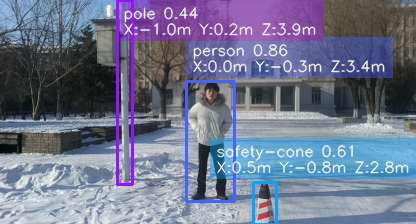
\includegraphics[width=\textwidth]{figures/chapter05/实地测距效果图_1.jpg}
  \end{minipage}
  \hfill
  \begin{minipage}[t]{0.49\textwidth}
    \centering
    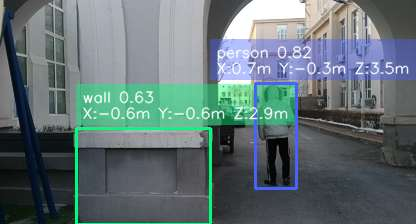
\includegraphics[width=\textwidth]{figures/chapter05/实地测距效果图_2.jpg}
  \end{minipage}
  \caption{实地测距效果图}
  \label{实地测距效果图}
\end{figure}

真实距离采用手持式激光测距仪进行测量，其标称精度为$\pm 3$ mm。测量时以相机光心为起点，选取目标可见表面的几何中心作为测量点，以保证与视觉测距输出的空间定义保持一致。对于每一类障碍物在每一个距离处的测距结果，均在目标对象及场景布置保持不变的条件下重复测量5次，用于检查读数稳定性，并记录稳定输出结果作为该距离下的视觉测距结果；激光测距仪测得距离作为参考真值，用于评估双目测距结果的误差。

\begin{table}[htbp]
  \centering
  \caption[不同类别障碍物在各距离下的测距结果与相对误差]{不同类别障碍物在各距离下的测距结果与相对误差}
  \label{不同类别障碍物在各距离下的测距结果与相对误差}
  \vspace{0.5em}\wuhao
  \begingroup
  \setlength{\tabcolsep}{3pt}
  \begin{thesistabular}{ccccccc}
    \toprule
    ID & 障碍物 & 2m & 4m & 6m & 8m & 10m \\
    \midrule
    1 & 行人 & 2.02(1.0\%) & 3.93(1.8\%) & 6.09(1.5\%) & 8.46(5.8\%) & 10.74(7.4\%) \\
    2 & 汽车 & 1.99(0.5\%) & 4.03(0.8\%) & 5.93(1.2\%) & 8.11(1.4\%) & 10.52(5.2\%) \\
    3 & 摩托车 & 1.93(3.5\%) & 4.19(4.8\%) & 5.71(4.8\%) & 8.40(5.0\%) & 9.19(8.1\%) \\
    4 & 路障 & 2.04(2.0\%) & 3.88(3.0\%) & 6.15(2.5\%) & 8.43(5.4\%) & 10.86(8.6\%) \\
    5 & 杆体 & 1.98(1.0\%) & 4.13(3.3\%) & 5.67(5.5\%) & 8.44(5.5\%) & 9.43(5.7\%) \\
    6 & 树木 & 2.01(0.5\%) & 3.94(1.5\%) & 6.05(0.8\%) & 8.34(4.3\%) & 10.43(4.3\%) \\
    \bottomrule
  \end{thesistabular}
  \endgroup
\end{table}

\begin{figure}[htbp]
  \centering
  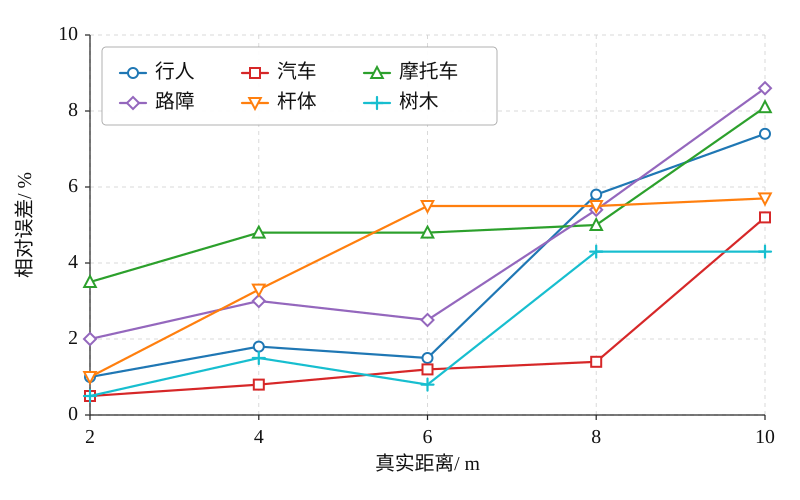
\includegraphics[width=0.95\textwidth]{figures/chapter05/不同类别障碍物相对误差折线图.pdf}
  \caption{不同类别障碍物相对误差随距离变化}
  \label{不同类别障碍物相对误差随距离变化}
\end{figure}

由表\ref{不同类别障碍物在各距离下的测距结果与相对误差}和图\ref{不同类别障碍物相对误差随距离变化}可知，在全部30组测量数据中，最大相对误差为8.6\%，出现在路障$10\,\mathrm{m}$测距条件下。不同距离下的最大相对误差分别为：$2\,\mathrm{m}$为3.5\%、$4\,\mathrm{m}$为4.8\%、$6\,\mathrm{m}$为5.5\%、$8\,\mathrm{m}$为5.8\%、$10\,\mathrm{m}$为8.6\%。按照前文提出的分阶段最大相对误差指标进行评价，系统在$2\sim4\,\mathrm{m}$近距离、$6\sim8\,\mathrm{m}$中距离和$10\,\mathrm{m}$远距离下的最大相对误差分别低于5\%、6\%和10\%，满足障碍物测距精度要求。

可以看出，测距误差随距离增加总体呈上升趋势。这一现象主要源于远距离条件下视差分辨率下降，导致深度量化误差增大。从单个目标看，摩托车在$2\,\mathrm{m}$处的相对误差为3.5\%，杆体在$6\,\mathrm{m}$处的相对误差为5.5\%，均属于对应距离条件下的较大误差样本。分析认为，上述误差波动与目标结构特征及当前采用的“ROI缩放+区域深度中位数”策略有关：当缩放后的感兴趣区域覆盖摩托车中心空腔时，部分背景深度值可能被纳入统计；而杆体等细长目标的有效深度区域较窄，也更容易受到背景深度干扰，从而影响代表性深度的计算结果。该问题表明，在中空结构目标和细长目标上仍存在一定优化空间，后续可通过前景分割或自适应深度筛选策略进一步提升测距稳定性。

\section{两轮平衡车自主行驶能力的测试实验}

在完成两轮平衡车行驶性能与环境感知能力的独立验证后，进一步开展整车自主行驶实验，验证系统各模块的协同工作效果与整体运行稳定性。本节分别从定位效果与动态避障能力两个方面对系统自主行驶性能进行测试与分析。

\subsection{卡尔曼滤波定位测试}

系统运行后，基于卡尔曼滤波的融合定位效果如图\ref{卡尔曼融合定位效果图}所示。在GPS出现波动的直角拐弯路段，融合定位能够滤除干扰并输出平稳位姿信息。

\begin{figure}[h]
\centering
\includesvg[width=0.85\textwidth]{figures/chapter05/卡尔曼融合定位效果图.svg}
\caption{卡尔曼融合定位效果图}
\label{卡尔曼融合定位效果图}
\end{figure}

实验过程中，融合定位结果以$120\,\mathrm{Hz}$频率持续输出，能够满足自动行驶对定位实时性的要求。由于实验场景缺乏高精度轨迹真值，进一步从轨迹几何连续性角度对融合定位结果进行分析。

为评价轨迹横向抖动程度，采用滑动窗口局部直线拟合方法。在第$i$个窗口内利用PCA得到局部拟合直线$l_i:a_i x+b_i y+c_i=0$，并将轨迹点$(x_i,y_i)$到该直线的正交距离定义为局部残差：
\begin{equation}
\label{eq:ch5-local-residual}
r_i=\frac{|a_i x_i+b_i y_i+c_i|}{\sqrt{a_i^2+b_i^2}}
\end{equation}
\begin{tabularx}{\textwidth}{@{}l@{\quad}r@{———}X@{}}
式中& $r_i$ & 第$i$个轨迹点的局部残差；\\
& $a_i,b_i,c_i$ & 第$i$个窗口内局部拟合直线的参数；\\
& $x_i,y_i$ & 第$i$个轨迹点的坐标。\\
\end{tabularx}\vspace{3.15bp}

局部残差变化如图\ref{定位残差位移对比}所示，统计结果见表\ref{局部残差统计结果对比}。GPS曲线在多个区段出现明显尖峰，点序号约600处残差突增至0.10\,m以上；融合结果整体幅值较低，仅局部轻微波动。表\ref{局部残差统计结果对比}显示，融合残差标准差降至0.003837\,m，约为GPS的35\%，最大残差降至0.027489\,m，表明融合定位有效抑制了轨迹横向抖动与异常波动。

\begin{figure}[htbp]
\centering
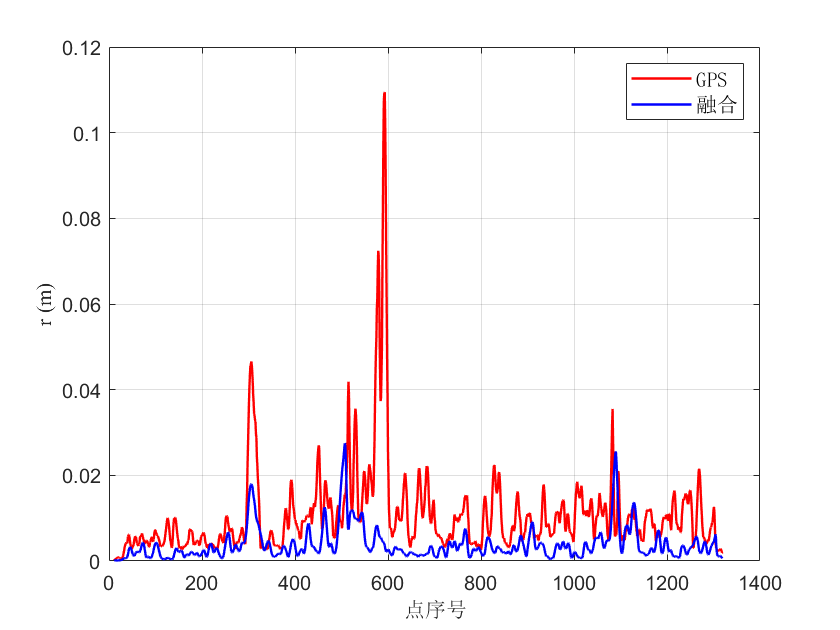
\includegraphics[width=1\textwidth]{figures/chapter05/定位残差位移.png}
\caption{局部残差变化对比}
\label{定位残差位移对比}
\end{figure}

\begin{table}[htbp]
  \centering
  \caption[局部残差统计结果对比]{局部残差统计结果对比}
  \label{局部残差统计结果对比}
  \vspace{0.5em}\wuhao
  \begin{thesistabular}{ccc}
    \toprule
    指标 & GPS(m) & 融合结果(m) \\
    \midrule
    均值 & 0.010786 & 0.003870 \\
    标准差 & 0.010941 & 0.003837 \\
    95\%分位 & 0.026327 & 0.011431 \\
    最大值 & 0.109462 & 0.027489 \\
    \bottomrule
  \end{thesistabular}
\end{table}

进一步对相邻轨迹方向变化进行分析。设相邻位置点为$(x_{i-1},y_{i-1})$和$(x_i,y_i)$，则轨迹方向角可表示为：
\begin{equation}
\label{eq:ch5-heading-angle}
\theta_i=\operatorname{atan2}(y_i-y_{i-1},x_i-x_{i-1})
\end{equation}
\begin{tabularx}{\textwidth}{@{}l@{\quad}r@{———}X@{}}
式中& $\theta_i$ & 第$i$段轨迹的方向角；\\
\end{tabularx}\vspace{3.15bp}
为消除角度周期性带来的不连续性，将相邻方向变化量归一化为：
\begin{equation}
\label{eq:ch5-heading-diff}
\Delta\theta_i=\operatorname{atan2}\bigl(\sin(\theta_i-\theta_{i-1}),\cos(\theta_i-\theta_{i-1})\bigr)
\end{equation}
\begin{tabularx}{\textwidth}{@{}l@{\quad}r@{———}X@{}}
式中& $\Delta\theta_i$ & 相邻两段轨迹的方向变化量。\\
\end{tabularx}\vspace{3.15bp}

以$|\Delta\theta_i|$评价轨迹方向连续性，其结果如图\ref{相邻方向变化绝对值对比}所示，统计结果见表\ref{方向变化统计结果对比}。从图中可以看出，GPS曲线在约300--500和1080--1300点区间出现持续的大幅振荡，并伴随接近$\pm 3\,\mathrm{rad}$的尖峰；融合结果大部分时间保持在零附近，仅在个别转向位置出现较小起伏。结合表\ref{方向变化统计结果对比}可知，融合结果的方向变化标准差由0.957\,rad降至0.070\,rad，95\%分位由1.728\,rad降至0.051\,rad，说明融合定位显著减小了局部方向摆动，轨迹连续性与平滑性明显提升。

\begin{figure}[htbp]
\centering
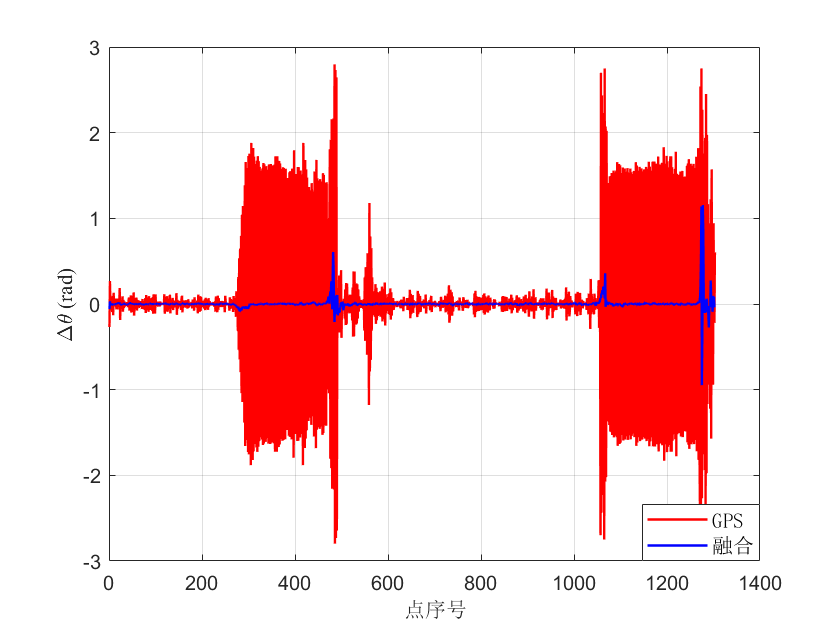
\includegraphics[width=1\textwidth]{figures/chapter05/相邻方向变化绝对值对比rad.png}
\caption{相邻方向变化量对比}
\label{相邻方向变化绝对值对比}
\end{figure}

\begin{table}[htbp]
  \centering
  \caption[方向变化统计结果对比]{方向变化统计结果对比}
  \label{方向变化统计结果对比}
  \vspace{0.5em}\wuhao
  \begin{thesistabular}{ccc}
    \toprule
    指标 & GPS(rad) & 融合结果(rad) \\
    \midrule
    标准差 & 0.957 & 0.070 \\
    绝对变化均值 & 0.599 & 0.016 \\
    95\%分位 & 1.728 & 0.051 \\
    \bottomrule
  \end{thesistabular}
\end{table}

\subsection{动态避障能力测试}

实验构建动态行人干扰场景。车辆按照预设目标点进行路径规划并开始正常行驶，在行驶过程中，行人从侧方突然进入车辆原规划路径，如图\ref{避障能力测试}所示。该场景模拟公园或园区环境中常见的行人随机横穿道路情形，对系统实时感知与动态避障能力提出挑战。

\begin{figure}[htbp]
  \centering
  \begin{minipage}[t]{0.32\textwidth}
    \centering
    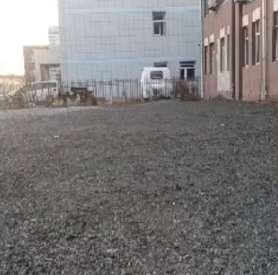
\includegraphics[width=\textwidth]{figures/chapter05/避障能力测试_1.jpg}
  \end{minipage}
  \hfill
  \begin{minipage}[t]{0.32\textwidth}
    \centering
    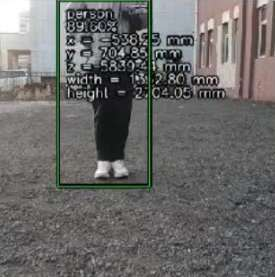
\includegraphics[width=\textwidth]{figures/chapter05/避障能力测试_2.jpg}
  \end{minipage}
  \hfill
  \begin{minipage}[t]{0.32\textwidth}
    \centering
    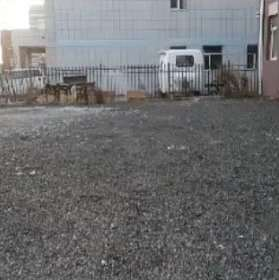
\includegraphics[width=\textwidth]{figures/chapter05/避障能力测试_3.jpg}
  \end{minipage}
  
  \vspace{0.6em}
  
  \begin{minipage}[t]{0.32\textwidth}
    \centering
    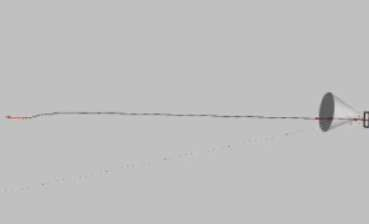
\includegraphics[width=\textwidth]{figures/chapter05/避障能力测试_4.jpg}
  \end{minipage}
  \hfill
  \begin{minipage}[t]{0.32\textwidth}
    \centering
    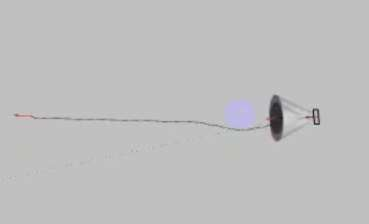
\includegraphics[width=\textwidth]{figures/chapter05/避障能力测试_5.jpg}
  \end{minipage}
  \hfill
  \begin{minipage}[t]{0.32\textwidth}
    \centering
    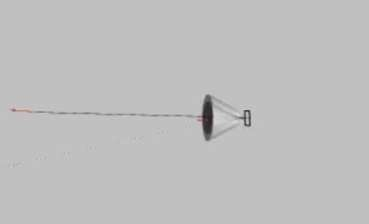
\includegraphics[width=\textwidth]{figures/chapter05/避障能力测试_6.jpg}
  \end{minipage}
  \caption{避障能力测试}
  \label{避障能力测试}
\end{figure}

实验过程中主要通过现场观察与图像序列记录车辆对动态行人的响应过程。结果表明，在设定行驶速度范围内，规划控制环节能够维持$20\,\mathrm{Hz}$的运行频率；当行人进入原规划路径后，系统能够识别前方动态障碍并触发局部路径调整，车辆在安全范围内表现出减速和绕行动作，未观察到明显失稳现象。

在个别情况下（如行人距离较近或横向移动较快），车辆会出现短暂停顿、减速或轻微轨迹调整不连续现象。结合系统运行机制分析，这可能与动态障碍物位置变化引起代价地图更新和局部规划重复计算有关。总体而言，该实验表明系统能够对动态行人干扰作出避让响应，具备动态障碍处理能力。

\section{本章小结}

本章对两轮平衡车的运动性能、视觉感知能力及自主行驶能力进行了综合实验验证。结果表明，所设计的两轮平衡车能够稳定完成基本行驶与复杂路径运动，验证了整车结构与控制系统的可靠性；双目视觉感知系统能够实现较稳定的障碍物检测与距离估计，满足自主行驶的环境感知需求；自主行驶实验表明，系统在定位波动和动态障碍干扰条件下能够进行路径调整与避让响应，验证了整车自主行驶方案的可行性。
